\section{Introduction}
Estimated Time of Arrival (ETA) prediction is a fundamental component of modern navigation systems and intelligent transportation applications. Accurate ETA enables commuters to make informed travel decisions, supports fleet management and logistics operations, and reduces congestion by distributing demand across the road network. With the ubiquity of GPS-enabled devices and connected vehicles, navigation platforms such as Google Maps and Waze \cite{derrowpinion2021googlemaps,hoseinzadeh2020waze,amin-naseri2018waze} have transformed how travelers plan and adapt their journeys. Despite this progress, ETA estimation remains challenging due to the dynamic and stochastic nature of urban traffic (see Fig.~\ref{fig:rush-hour-intro}).

\begin{figure*}[t]
    \centering
    \IfFileExists{figures/rush_hour.png}{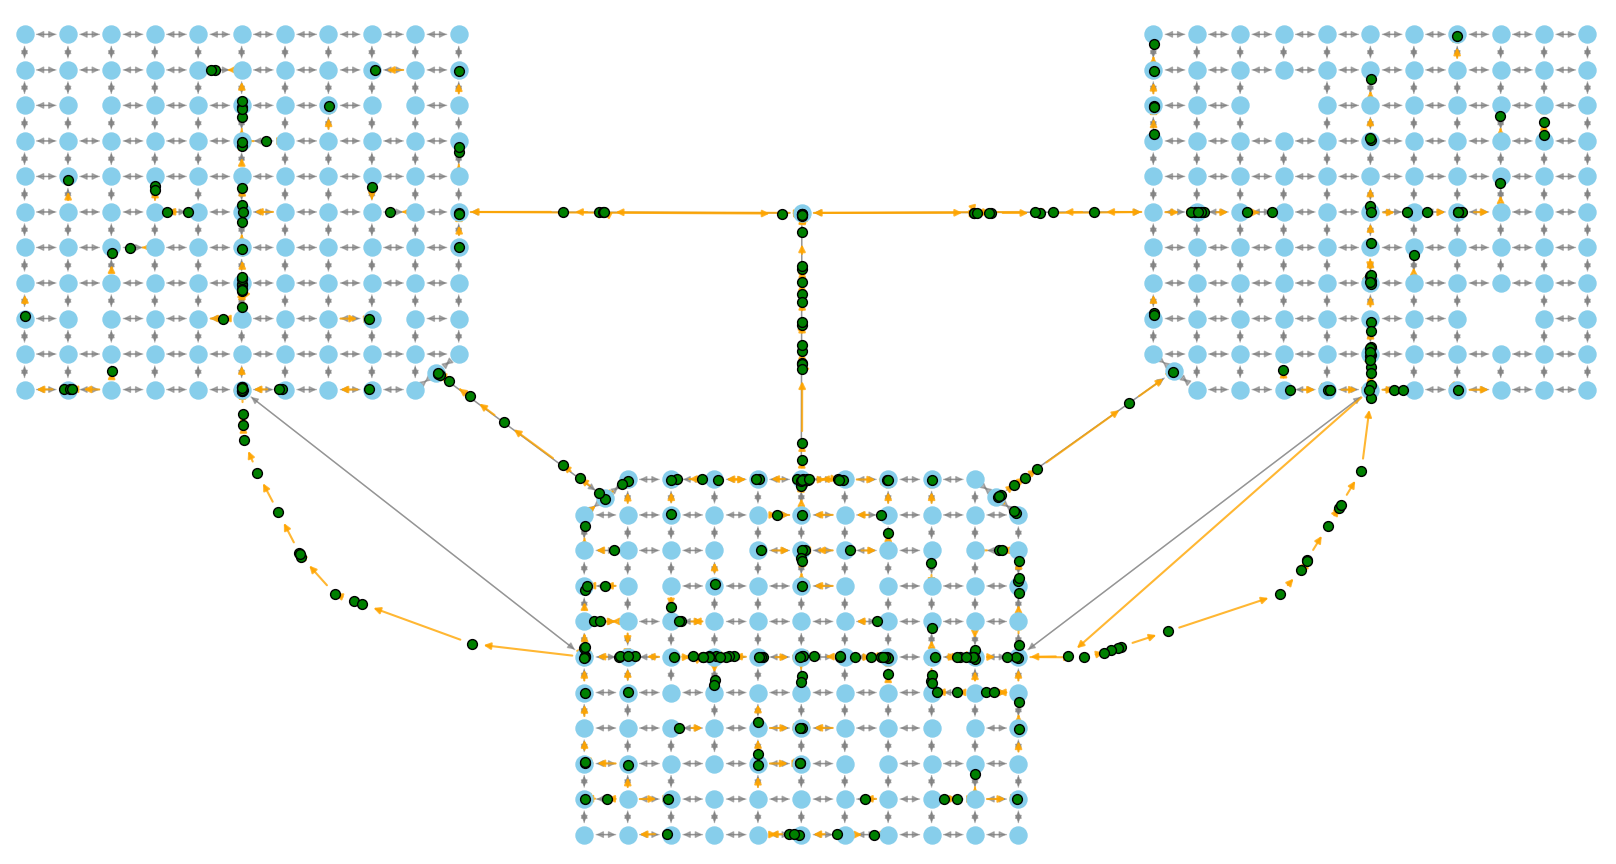
\includegraphics[width=0.80\textwidth]{figures/rush_hour.png}}{\fbox{\parbox{0.80\textwidth}{\centering Rush-hour snapshot placeholder}}}
    \caption{Afternoon rush-hour snapshot spanning the network. Static junction nodes (light blue) and static road edges (gray) form the backbone; dynamic vehicle nodes (green) and traversal edges (orange arrows) reveal congestion corridors and high-flow funnels. Zones: A/B urban grids with dense signals and short links; C suburban ring with longer arterials and smoother flow; H connector hub that funnels inter-zone traffic and creates gateway bottlenecks.}
    \label{fig:rush-hour-intro}
\end{figure*}

Traditional approaches rely on shortest-path algorithms such as Dijkstra's algorithm \cite{dijkstra1959}, which efficiently compute routes under static conditions but fail to capture evolving congestion or vehicle interactions. As a result, travel times obtained from such methods can diverge substantially from reality when conditions change during a trip.

With the growth of urban mobility datasets, machine-learning models have been applied to ETA prediction. Tree-based methods such as XGBoost \cite{chen2016xgboost} leverage handcrafted features and perform well on aggregated trip records, including NYC Taxi and Porto Taxi \cite{nyc_tlc,moreira2013porto}. Deep learning approaches improve accuracy by modeling temporal patterns and spatio-temporal context along a route. For example, DeepTTE learns ETA from raw GPS traces \cite{deepTTE2018}, TADNM incorporates transportation-mode awareness \cite{xu2020tadnm}, MetaTTE applies meta-learning for cross-city generalization \cite{wang2022metatte}, and STAD corrects routing-engine outputs using spatio-temporal adjustments \cite{abbar2020stad}.

In parallel, graph-based spatio-temporal learning has advanced traffic prediction by representing road networks as graphs and capturing dynamics through diffusion or convolution operators (e.g., DCRNN, ST-GCN, Graph WaveNet) \cite{dcrnn2018,yu2018stgcn,wu2019graphwavenet}. However, existing benchmarks such as NYC, Porto, Chengdu/DiDi, and Geolife \cite{nyc_tlc,moreira2013porto,didi2016,zheng2012geolife} lack explicit representation of pre-planned routes. Models must therefore infer likely paths between origin and destination, introducing ambiguity and reducing accuracy. 

To address this limitation, we represent traffic as a dynamic, multi-relational graph in which static junction-to-junction road edges are complemented by time-varying vehicle and interaction edges (see Fig.~\ref{fig:dyn-graph}). This formulation builds on our earlier research in traffic simulation and route-aware modeling \cite{voloch2021,SmartSimulativeRoute2025}, which laid the methodological groundwork for graph-based analysis of traffic dynamics. In the present work, we advance this foundation by explicitly encoding each vehicle's remaining planned route (route intent) and by learning temporal context from stable road edges across recent history, while leveraging the complete dynamic graph at the final snapshot to predict per-vehicle ETA.

\noindent\textbf{Results.} On a four-week urban simulation, a simple average-time baseline attains 260.6\,s MAE; our route-aware non-temporal variant achieves 58.4\,s MAE, and the temporal route-aware model reaches 46.2\,s MAE. These gains highlight the value of making route intent explicit and of learning temporal signals from stable road infrastructure rather than noisy, transient vehicle interactions.

\noindent\textbf{Paper outline.} We introduce the dynamic graph representation and problem setup, summarize dataset characteristics and splits, detail the model architecture, and then present experiments and ablations followed by discussion and conclusions. To ground the setting early, Fig.~\ref{fig:rush-hour-intro} provides a system-level rush-hour snapshot.

\noindent\textbf{Contributions.} We introduce a dynamic, multi-relational traffic graph that unifies static junction nodes and road edges with dynamic vehicle nodes and interaction edges, and we provide explicit remaining-route annotations per vehicle to expose route intent. Building on this representation, we design a route-aware spatio-temporal GNN that learns temporal context from stable road edges over the first $H{-}1$ snapshots and fuses it with full-graph features at prediction time using a sparse Mixture-of-Experts head for specialization. 
% removed two-panel intro figure per request
